\begin{figure}[H]
	\centering
	\setlength{\fboxsep}{0 cm}
	\fbox{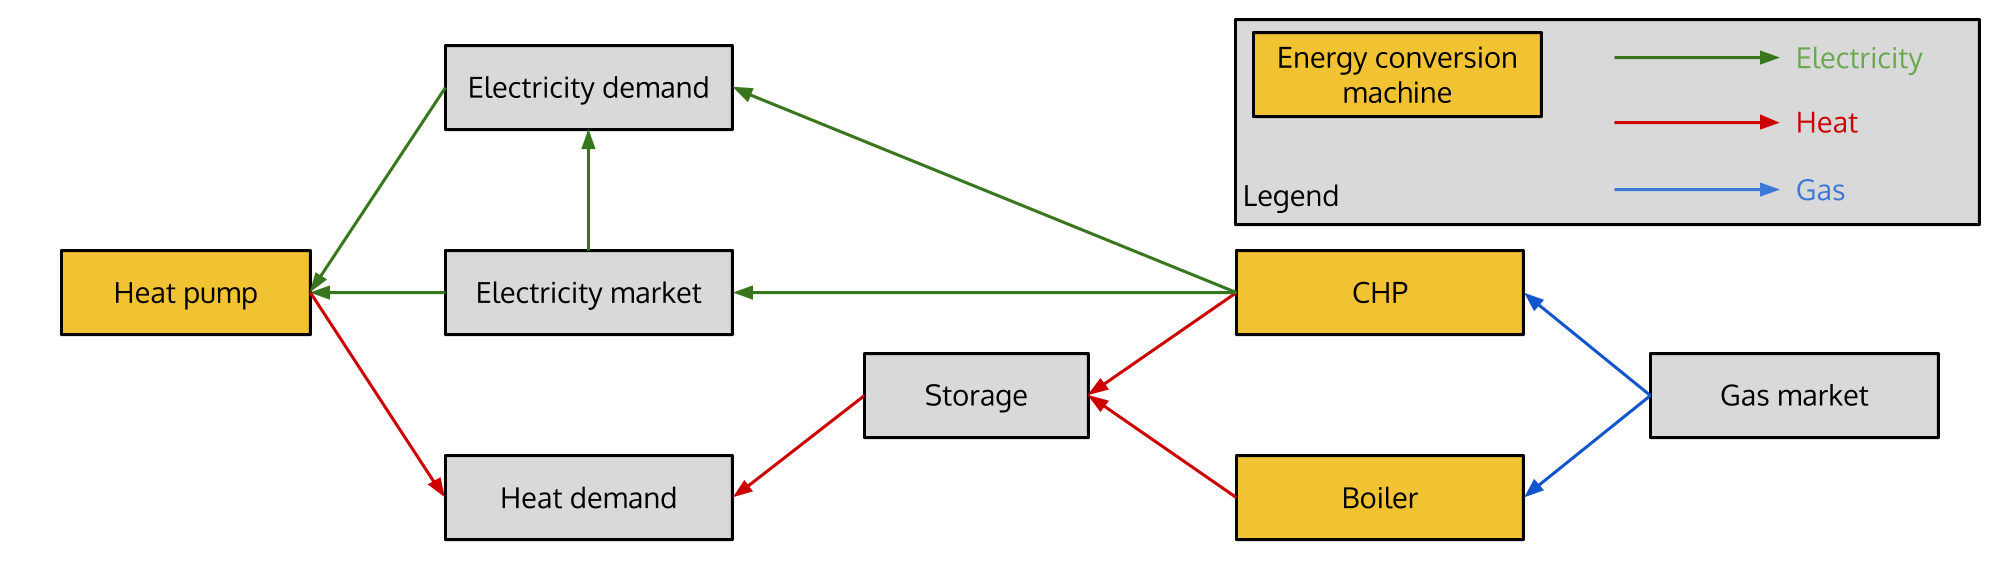
\includegraphics[width=17cm]{Images/FlowchartGeneral.png}}
	\setlength{\fboxsep}{0.1 cm}
	\caption{An overview of the general system model. One can see the different energy streams (electricity, green; heat, red; gas, blue).}
	\label{F:GeneralFlowshart}
\end{figure}

\begin{eqnarray}
\text{Electrical efficiency} &=& \frac{\text{Electrical output} [\unit{kW}]}{\text{Fuel input} [\unit{kW}]}\\
\text{Overall efficiency} &=& \frac{\text{Heat} + \text{Electrical output} [\unit{kW}]}{\text{Fuel input} [\unit{kW}]}
\end{eqnarray}